\documentclass{homework}
\usepackage{ctex}
\usepackage{bm}
\usepackage{makecell}
\usepackage[ruled,vlined]{algorithm2e}
\usepackage{booktabs}
\usepackage{multirow}
\usepackage{siunitx}
\usepackage{graphicx}
\usepackage{amsmath}
\usepackage{subcaption}
\usepackage{caption}
\newcommand{\bfx}{\mathbf{x}}
\newcommand{\bfg}{\mathbf{g}}
\newcommand{\bfH}{\mathbf{H}}
\newcommand{\bfd}{\mathbf{d}}
\author{李健宁}
\class{机器学习中的优化问题}
\date{\today}
\title{Homework 14}
% \address{Bayt El-Hikmah}

\graphicspath{{./media/}}

\begin{document} \maketitle

\question

\begin{sol}
应用题目中要求的几种方法,最大迭代次数$1000$次,学习率$\eta = 0.01$,其他参数采取Pytorch中相应优化器的默认参数,实验结果如图\ref{1}。

\begin{figure}[h]
    \centering
    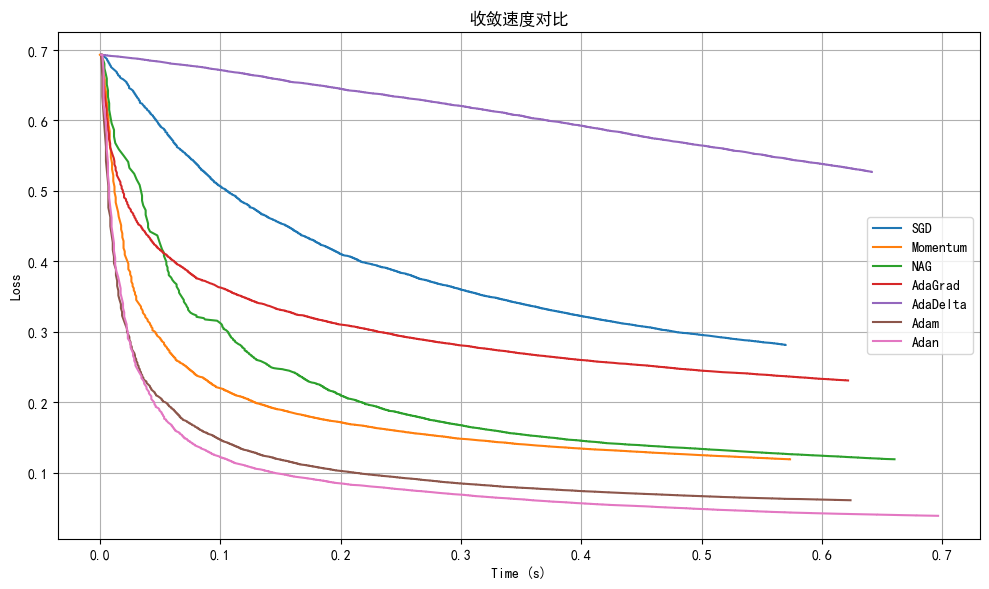
\includegraphics[width=0.5\linewidth]{1.png}
    \caption{收敛速度对比}
    \label{1}
\end{figure}

\end{sol}

% \begin{figure}[h]
%     \centering
%         \centering
%         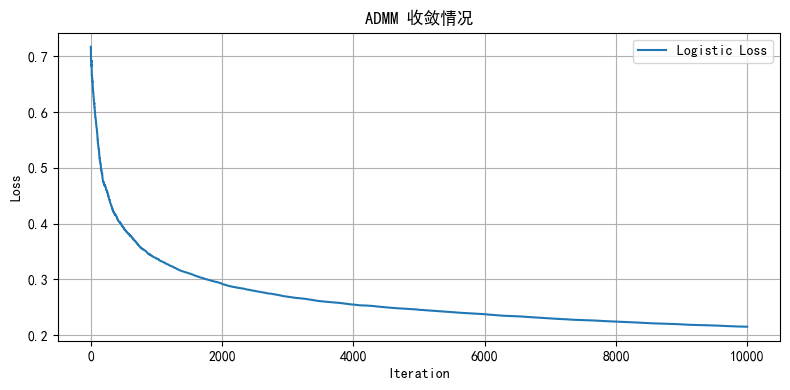
\includegraphics[width=0.8\linewidth]{4.png}
%         \caption{LADMPSAP收敛行为}\label{4}
% \end{figure}

\question
\begin{sol}
    
在 RCD(1) 方法中,我们对每个坐标 \( i \) 维护一个自适应步长缩放因子 \( \beta_i \),其估计采用指数滑动平均方式,具体更新如下
\begin{equation}
\beta_i^{(t)} = \rho \cdot \beta_i^{(t-1)} + (1 - \rho) \cdot \left( \nabla_i f(w^{(t-1)}) \right)^2
\end{equation}

其中\( \rho \in [0,1) \) 是滑动平均系数,这里取\( \rho = 0.9 \); \( \nabla_i f(w^{(t-1)}) \) 表示在第 \(t-1\) 次迭代中,第 \(i\) 个分量的梯度; \( \beta_i^{(t)} \) 表示当前估计的第 \(i\) 个分量的尺度。

最大迭代次数$1000$次,学习率$\eta = 0.01$,其他参数采取Pytorch中相应优化器的默认参数,实验结果如图\ref{2}。

\begin{figure}
    \centering
    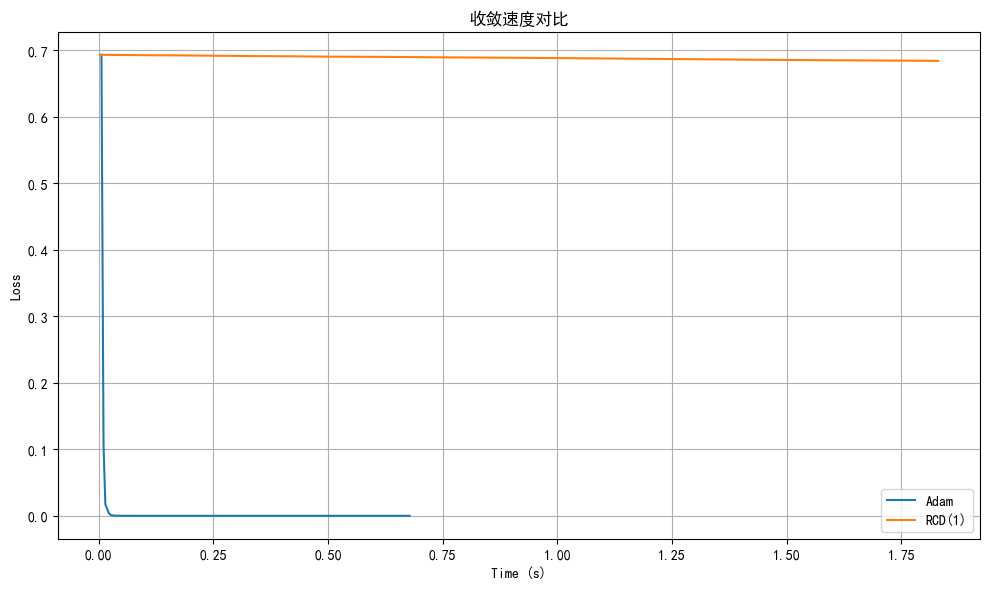
\includegraphics[width=0.5\linewidth]{2.png}
    \caption{收敛速度对比}
    \label{2}
\end{figure}
\end{sol}

\question

\begin{sol}
    为引入 ADMM 结构,我们将变量 \(\bm{w}\) 分裂为两个变量 \(\bm{w}\) 与 \(\bm{z}\),得到等价问题
\begin{align*}
\min_{\bm{w}, \bm{z}} \quad & \frac{1}{N} \sum_{i=1}^N \log\left(1 + \exp\left(-y_i \cdot \bm{x}_i^\top \bm{w}\right)\right) \\
\text{s.t.} \quad&A_1w+A_2z = b,\\
A_1 = \begin{bmatrix}
I_d \\
\bm{0}^\top
\end{bmatrix} \in \mathbb{R}^{(d+1) \times d},\,
A_2 &= \begin{bmatrix}
- I_d \\
\bm{1}^\top
\end{bmatrix} \in \mathbb{R}^{(d+1) \times d},\,
b   = \begin{bmatrix}
\bm{0} \\
1
\end{bmatrix} \in \mathbb{R}^{(d+1)}
\end{align*}

每次迭代的具体更新方式,首先随机选取样本索引$i_k \in \{1, 2, \dots, N\}$,然后根据以下公式依次更新
\begin{align}
w^{k+1} &= \arg\min_w \left\{ \nabla f_{i_k}(w^k)^\top (w - w^k) + \frac{\rho}{2} \left\| A_1 w + A_2 z^k - b + \frac{1}{\rho} u^k \right\|^2 + \frac{1}{2 \eta_k} \left\| w - w^k \right\|^2 \right\} \label{eq:update_w} \\
z^{k+1} &= \arg\min_z \left\{ I_{\{\mathbf{1}^\top z = 1\}}(z) + \frac{\rho}{2} \left\| A_1 w^{k+1} + A_2z - b + \frac{1}{\rho} u^k \right\|^2 \right\} \label{eq:update_z} \\
u^{k+1} &= u^k + \rho \left( A_1 w^{k+1} + A_2 z^{k+1} - b \right) \label{eq:update_u}
\end{align}

参数选取上,惩罚参数$\rho = 0.1$,初始学习率$\eta_0 = 0.1$, $\eta_k = \frac {\eta_0}{\sqrt{k+1}}$,最大迭代次数$10000$次,实验结果如图\ref{3},\ref{4}。

\begin{figure}[h]
    \centering
    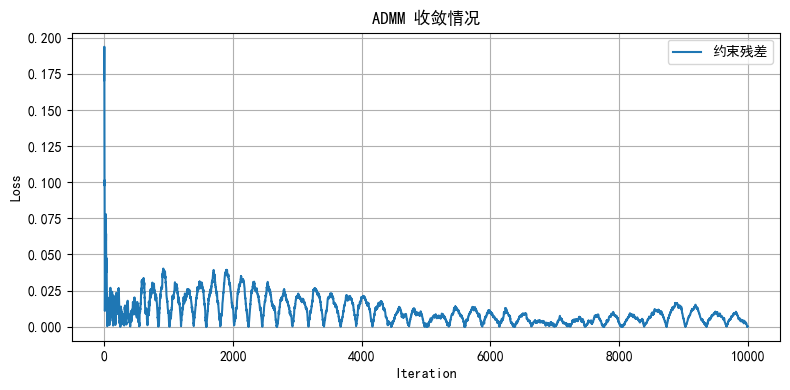
\includegraphics[width=0.6\linewidth]{3.png}
    \caption{约束残差$\|A_1w+A_2z - b\|$}
    \label{3}
\end{figure}

\begin{figure}[h]
    \centering
    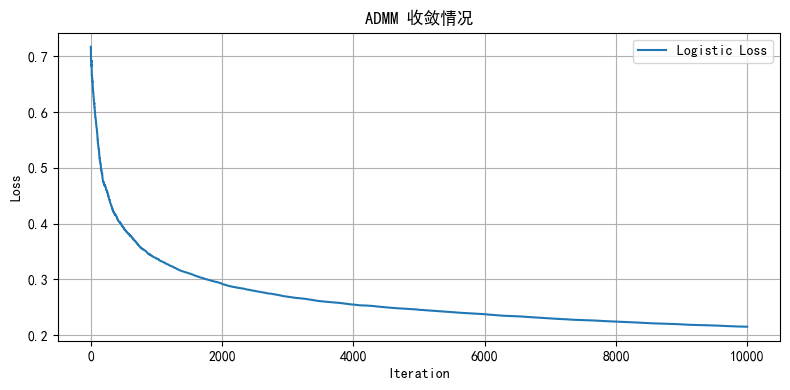
\includegraphics[width=0.6\linewidth]{4.png}
    \caption{Logistice Loss(目标函数值)}
    \label{4}
\end{figure}

\end{sol}

% \bibliographystyle{plain}
% \bibliography{citations}

\end{document}
